\documentclass[10pt,a4paper]{article}
\usepackage[utf8]{inputenc}
\usepackage[german]{babel}
\usepackage[T1]{fontenc}
\usepackage{amsmath}
\usepackage{amsfonts}
\usepackage{amssymb}
\usepackage{makeidx}
\usepackage{graphicx}
\usepackage[left=2cm,right=2cm,top=2cm,bottom=2cm]{geometry}
\usepackage{float}
\title{Korrektur Thermodynamik C14}
\author{Erik Zimmermann}
\begin{document}
\maketitle
\newpage
\section{Korrektur systematische Fehler}
Mit den vorher abgesprochenen Formeln für Gruppe 1:
\begin{align}
\sigma_T=\frac{2.7}{100}\cdot (T-T_{Eis})\\
\sigma_P=\frac{\sqrt{3}}{100}\cdot (P-P_{WStation})
\end{align}
und Gruppe 2:
\begin{align}
\sigma_T\approx 0\\
\sigma_P=\frac{\sqrt{3}}{100}\cdot (P-P_{WStation})
\end{align}
ergeben sich mit den korrigierten systematischen Fehlern folgende Tabellen:

\begin{table}[H]\centering
\caption{Ergebnisse Gruppe 1}

\begin{tabular}{c|c|c|c|c}
Abschnitt&T in K&$\Lambda$ in $\frac{kJ}{mol}$&$\sigma_{\Lambda_{stat}}$in $\frac{kJ}{mol}$&$\sigma_{\Lambda_{sys}}$in $\frac{kJ}{mol}$\\
\hline
1&366.37&41.74&0.342&1.043\\
2&363.81&42.08&0.327&1.052\\
3&361.65&43.27&0.339&1.082\\
4&359.72&41.62&0.324&1.041\\
5&358.0&42.51&0.327&1.063\\
6&356.39&43.34&0.294&1.084\\
7&354.95&42.88&0.272&1.073\\
8&353.53&42.65&0.365&1.067\\
9&352.27&41.19&0.327&1.031\\
10&351.06&44.01&0.384&1.102\\
11&349.95&41.45&0.395&1.038\\
12&348.87&41.2&0.299&1.032\\
13&347.84&42.88&0.406&1.075\\
14&346.86&45.11&0.432&1.131\\
15&345.91&39.82&0.446&0.999\\
16&344.99&40.41&0.414&1.014\\
17&343.32&41.56&0.143&1.044\\
18&342.4&38.78&0.163&0.975\\
19&341.57&42.03&0.212&1.057\\
20&340.68&36.24&0.175&0.914\\
21&339.78&37.06&0.189&0.935\\
\end{tabular}
\end{table}
\begin{table}[H]\centering
\caption{Ergebnisse Gruppe 2}

\begin{tabular}{c|c|c|c|c}
Abschnitt&T in K&$\Lambda$ in $\frac{kJ}{mol}$&$\sigma_{\Lambda_{stat}}$in $\frac{kJ}{mol}$&$\sigma_{\Lambda_{sys}}$in $\frac{kJ}{mol}$\\
\hline
1&367.93&42.18&0.273&0.008\\
2&364.13&41.17&0.156&0.017\\
3&360.76&41.96&0.102&0.026\\
4&357.71&40.97&0.1&0.036\\
5&355.03&41.8&0.12&0.045\\
6&352.6&42.24&0.117&0.055\\
7&350.38&42.31&0.136&0.065\\
8&348.4&43.03&0.141&0.074\\
9&346.54&42.79&0.162&0.084\\
10&344.83&40.84&0.175&0.094\\
\end{tabular}
\end{table}

Die besprochene Variation um die systematischen Fehler und das Einzeichnen des Literaturwerts ergibt für Gruppe 1:

\begin{figure}[H]
\centering
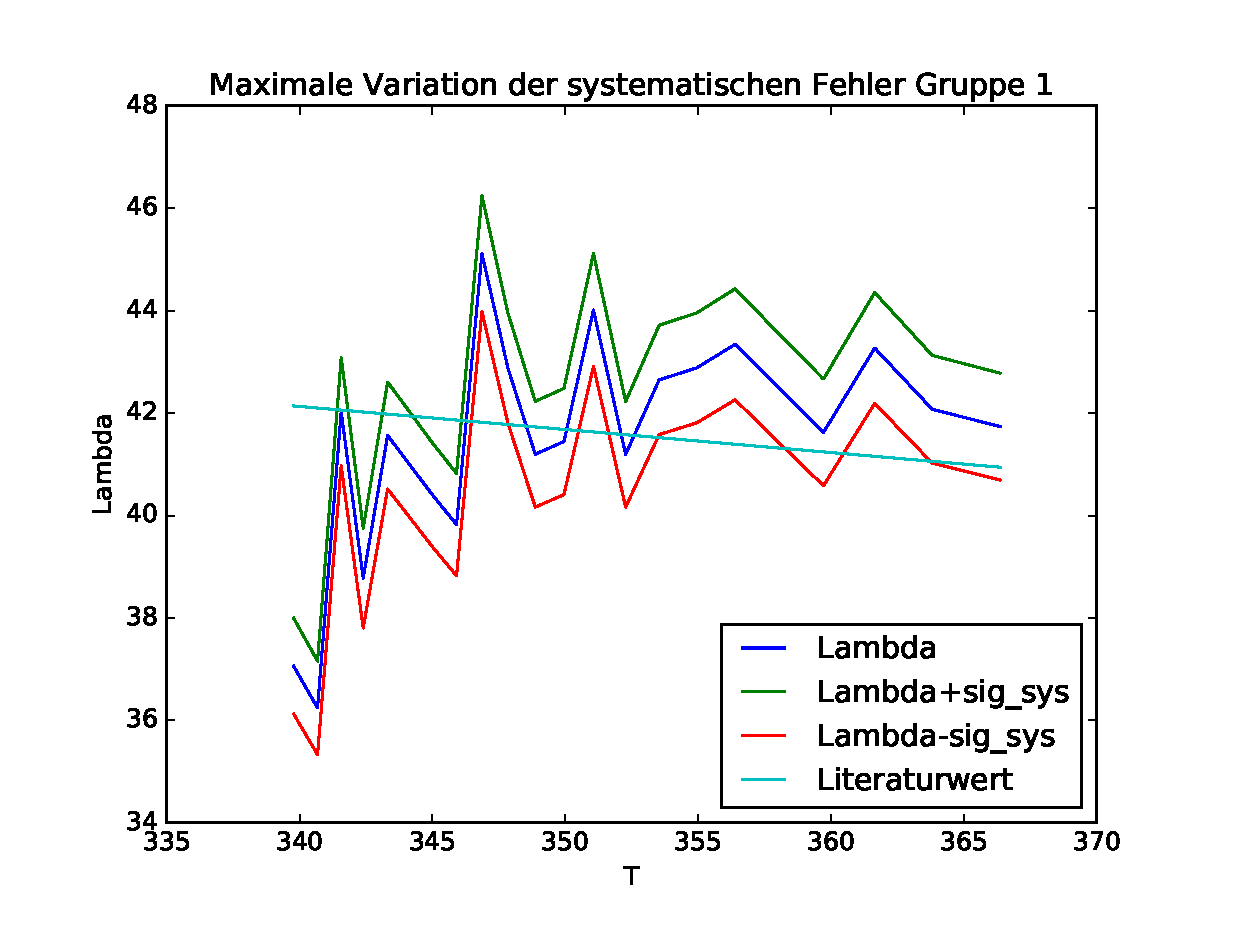
\includegraphics[scale=0.70]{Variation_sig_sys_G1.eps}
\caption{Verdampfungswärme gegen Temperatur Gruppe 1}
\end{figure}

und für Gruppe 2:
\begin{figure}[H]
\centering
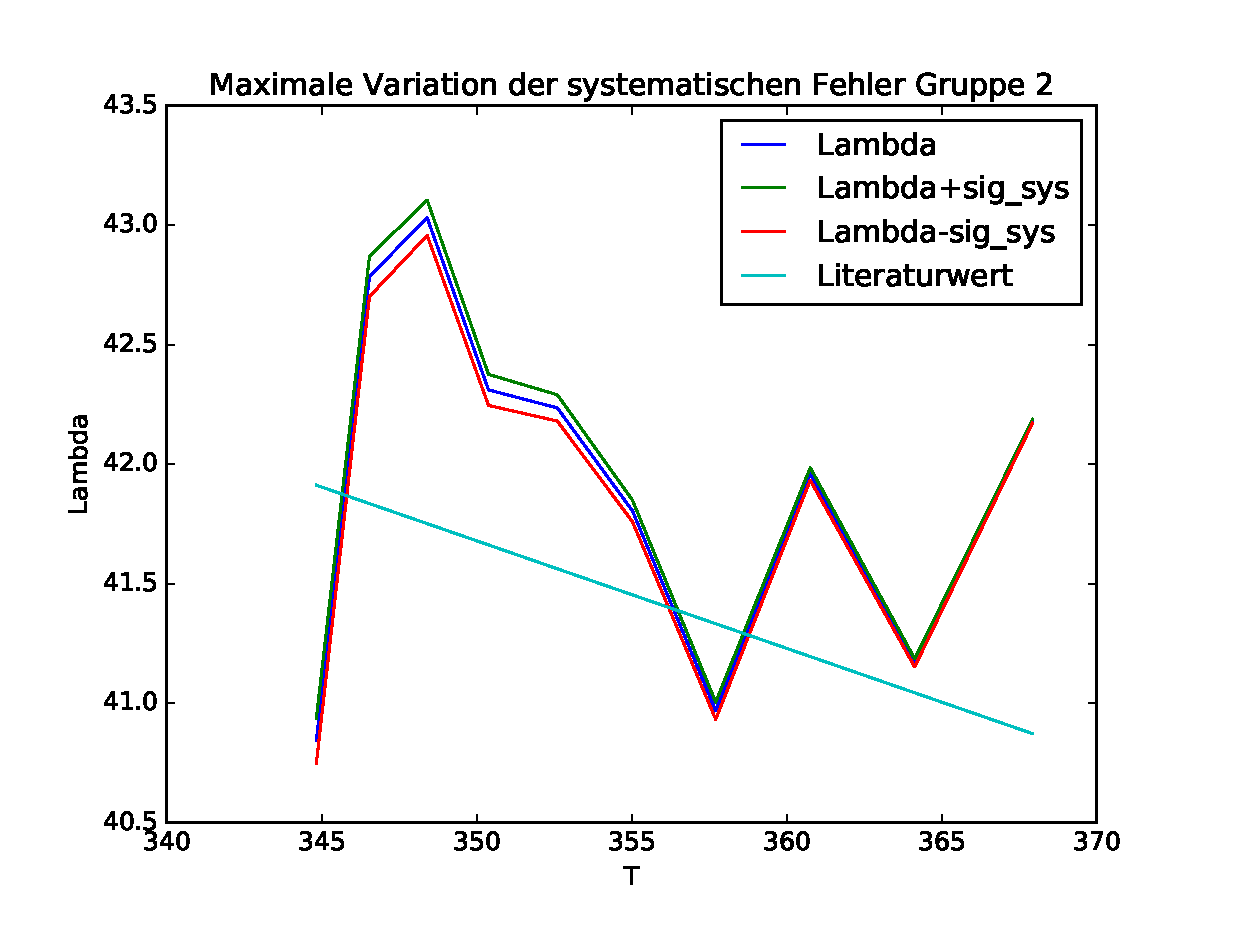
\includegraphics[scale=0.70]{Variation_sig_sys_G2.eps}
\caption{Verdampfungswärme gegen Temperatur Gruppe 2}
\end{figure}
Damit man überhaupt eine Verschiebung um $\sigma_{sys}$ erkennen kann, wurden bei Gruppe 2 (im Gegensatz zur Abbildung 22 im Bericht) die ersten und letzten Werte, so wie auch in der Auswertung, weggelassen.
\end{document}